\documentclass[twocolumn, amsmath]{revtex4}

\usepackage{graphicx}
\graphicspath{ {tex_pics/} }
\usepackage{siunitx}


\begin{document}

\title{PHYS 605 Lab\#5} 
\author{Evin O'Shea}  % fill in your name here
\author{Morgan Daly}
\email{eco2000@wildcats.unh.edu}  % add your email address 
\date{\today}  


\begin{abstract}
\end{abstract}

\maketitle



\section{Introduction and Theory}

\subsection{Purpose}
The goal of the lab was to construct different RC filters. The first part of the lab was to build an RC filter and take measurements of how it works as a low pass filter. The goal of the second part of the lab was to build another RC circuit with a slightly lower characteristic frequency and to take measurements to see how this could act as a high pass filter. After the low and high pass filters were built, they were casaded to create a band pass filter.


\subsection{Background / Theory} 
An RC circuit can be used as both a low pass filter and high pass filter. This is because the impedance of a capacitor is dependant on the frequency of the input voltage. As impedance of the circuits changes, the voltage across the capacitor also changes. When a load is connected to the capacitor, as the frequency varies, the voltage output to the load also changes. For lower frequencies, the voltage to the load will be small. This means the low frequencies are filtered out. A low pass RC filter is shown below:

\begin{figure}[h]  
	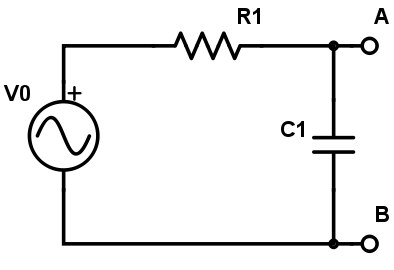
\includegraphics[scale = 0.2]{lowpassfilter.png}
	\caption{Design of the low pass filter.}
\end{figure}

The gain of the output of this circuit is governed by the equation shown below:

\begin{equation}
|G| = \frac{1}{(1 + (\omega RC))^{\frac{1}{2}}}
\end{equation}

The high pass filter works the same was as the low pass filter. The only difference is that the load is connected to the resistor. This just means that when the voltage across the capacitor is low, the voltage aross the resistor is high and when the volateg across the capacitor is high, the voltage across the resistor is low. A high pass RC filter is shown below:

\begin{figure}[h]  
	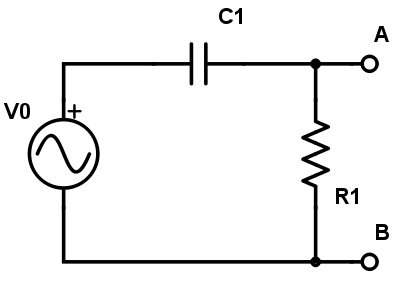
\includegraphics[scale = 0.2]{highpassfilter.png}
	\caption{Design of the high pass filter.}
\end{figure}

The gain of the output of the high pass filter is given by the equation below:

\begin{equation}
|G| = \frac{\omega RC}{(1 + (\omega RC)^2)^{\frac{1}{2}}}
\end{equation}

A band pass filter can be made by connecting the output of a low pass filter to the input of a high pass filter. This will cause both low and high voltages to be filtered out, leaving only middle range frequencies. This is because the low pass filter sends only  middle and low freqencies to the high pass filter and the high pass filter removes the low frequencies. A schematic of this type of band pass filter is shown below:

\begin{figure}[h]  
	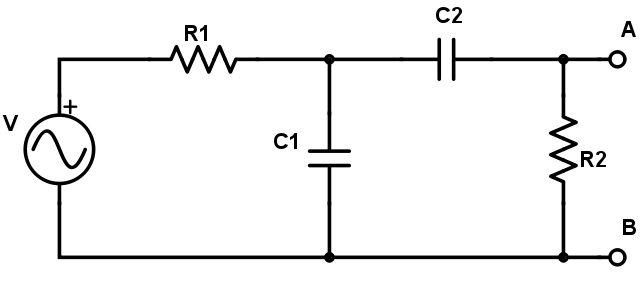
\includegraphics[scale = 0.2]{bandpassfilter.png}
	\caption{Design of the band pass filter.}
\end{figure}

The gain of two filters that are connected in this way is multiplicative:

\begin{equation}
|G| = G_{low}G_{high}
\end{equation

To make sure the middle frequencies make it through, there has to be overlap in the frequencies that are not filtered out. This is done by controlling the characteristic frequency of the low and high pass filters and offesetting them. The characteristic freqency is given by the equation below:

\begin{equation}
\omega _{RC} = \frac{1}{RC}
\end{equation

This frequency demonstrates when frequencies are filtered out by a filter. For a low pass filter, $\omega$ that are greater than $\omega _{RC}$ will be filtered out and for a high pass filter, $\omega$ that are less than $\omega _{RC}$ are filtered out. To mkaes the band pass filter, the $\omega _{RC}$ of the low pass filter was greater than the $\omega _{RC}$ for the high pass filter. This means that between these two values, frequencies will not be filtered out and the frequencies outside of this range will be filtered. This creates a band pass filter.

%should take it out if not calculating it
%\begin{equation}
%\phi = arctan(\frac{1}{\omega RC})
%\end{equation}


\section{Methodology}

% this is just procedure from lab 4
\begin{enumerate}
    \item Calculate the characteristic frequency of the low pass filter. Ensure that it is in the range of the signal generator being used.
    \item Construct the RC circuit as shown in Fig (1). Ensure that the total impedance is appropriate for the power source and oscilloscope.
    \item Connect the oscilloscope in parallel with the battery to monitor the input voltage, and in parallel with the capacitor to record the voltage drop across the capacitor, as well as the phase shift.
    \item Select an input voltage $V_{in}$ that will provide enough voltage to measure, but not exceed the power rating of the resistor.
    \item Measure and record the voltage drop, $V_{out}$, and the phase shift with respect to input, $\phi$ across the capacitor. 
    \item Repeat step (5) to obtain data for at least two decades above and below the resonant frequency.
    \item Calculate the characteristic frequency of the high pass filter. Ensure that it is lower than the characteristic frequency of the low pass filter.
    \item Construct the RC circuit as shown in Fig (2). Ensure that the total impedance is appropriate for the power source and oscilloscope.
    \item Connect the oscilloscope in parallel with the battery to monitor the input voltage, and in parallel with the resistor to record the voltage drop across the resistor, as well as the phase shift.
    \item Repeat step (5) to obtain data for at least two decades above and below the characteristic frequency.
    \item Connect the input of the high pass filter to the output of the low pass filter as shown in Fig. (3).
    \item Connect the oscilloscope in parallel with the battery to monitor the input voltage, and in parallel with the resistor to record the voltage drop across the resistor, as well as the phase shift.
    \item Repeat step (5) to obtain data for the same range used in the first two parts of the lab.
\end{enumerate}



\section{Results and Analysis}

\subsection{Data}
For the low pass filter, the expected characteristic frequency was f=5705.1Hz. This was obtained by using a 0.510nF capacitor and a 54.7k$\Omega$ resistor.
% why units in table instead of in column labels?
The data collected for the low pass filter is shown below:
\begin{center}
	\begin{ruledtabular}
    \begin{tabular}{ l l l l l }
    frequency (Hz)  & $V_{in} (mV)$ & $V_{out} (V)$ & $\phi (degrees)$\\ \colrule
 
    10.33  	& 4.56	& 4.32 & 0  \\
    66.67	& 4.6	& 4.40 & 0 \\ 
    100.7	& 4.6 	& 4.40 & 3   \\ 
    520.8	& 4.6 	& 4.32 & 7   \\ 
    1111 & 4.6 & 4.24 & 16	  \\ 
    3205 & 4.6 & 3.44 & 41	  \\ 
    5682 & 4.6 & 2.72 & 57	    \\ 
    8197 & 4.6 & 2.08 & 64	    \\ 
    10420  & 4.6 & 1.76 & 73	    \\
    60240 & 4.6 & 0.312 & 77	     \\ 
    108700 & 4.6 & 0.180 & 86	 \\
    \end{tabular}
    \end{ruledtabular}
\end{center}




For the high pass filter, the expected characteristic frequency was f=1896.3Hz. This was obtained by using a 1.526nF capacitor and a 55.0k$\Omega$ resistor.

The data collected for the high pass filter is shown below:

\begin{center}
	\begin{ruledtabular}
    \begin{tabular}{ l l l l l }
    \hline
    frequency (Hz)  & $V_{in} (mV)$ & $V_{out} (V)$ & $\phi (degrees)$\\ \colrule
 
    10.37  	& 4.48	& 0.036 & -80 \\ 
    60.24	& 4.6	& 0.152 & -86 \\ 
    106.4	& 4.6 	& 0.248 & -90   \\ 
    573.9	& 4.6 	& 1.44 & -71  \\ 
    862.1 	& 4.6 & 1.8 &   -60  \\ 
    1894 	& 4.6 & 3.04 & -43	  \\ 
    5618 	& 4.6 & 3.92 & -20	    \\ 
    6494 	& 4.6 & 4.00 & -18	    \\ 
    10310 	& 4.6 & 4.00 & -7	    \\ 
    46300 	& 4.6 & 4.00 & -3	     \\
    108700 	& 4.6 & 4.00 & 0	 \\
    \end{tabular}
    \end{ruledtabular}
\end{center}

The band pass filter was made of the low pass and high pass filters used in the first and second parts of the lab.
The data collected for the band pass filter is shown below:

\begin{center}
	\begin{ruledtabular}
    \begin{tabular}{ l l l l l }
    frequency  & $V_{in} (mV)$ & $V_{out} (V)$ & $\phi (degrees)$\\ \colrule
 
    10.33 	& 4.6	& 0.0296 & 	 \\ 
    68.49	& 4.6	& 0.168 & 	 \\
    108.7	& 4.6 	& 0.248 & 	   \\ 
    625.0	& 4.6 	& 1.24 & 	  \\ 
    1020 & 4.6 & 1.60 & -29	  	\\
    3425 & 4.6 & 1.84 & -25	    \\
    8197 & 4.6 & 1.44 & 41	    \\
    13160 & 4.6 & 1.12 &  53	    \\
    60240 & 4.6 & 0.272 & 82	     \\ 
    108700 & 4.6 & 0.163 & 89	 	\\
    \end{tabular}
    \end{ruledtabular}
\end{center}


\subsection{Calculations}

The gain in dB obtained from measurmens in the lab was caulculated using the equation:

\begin{equation}
Gain (dB) = 20log(\frac{V_{out}{V_{in}})
\end{equation}

A sample calculation for the gain for the low pass filter is:

\begin{equation}
Gain (dB) = 20log(\frac{4.32}{4.56}) = -0.4696 dB
\end{equation}

The expected gain was calculated using equations (1), (2), and (3) to find the magnitude of the gain and then taking the log of the gain and multiplying by twenty. For the same low pass filter data point as above the expected gain is:

\begin{equation}
Gain (dB) = 20log(\frac{1}{(1 + (\omega RC))^{\frac{1}{2}}}) = 20log(\frac{1}{(1 + (64.9 x 54.7x10^3 x 0.51x10^{-9}))^{\frac{1}{2}}}) -0.0079 dB
\end{equation}

The calculated data for the low pass filter is shown below:

\begin{center}
	\begin{ruledtabular}
    \begin{tabular}{ l l l l l }
    log(f)  & Gain (dB) & $Gain_{expected}$ (dB) & \% error \\ \colrule
 
    1.014  	&      -0.4696	& -0.0079	 & 	 \\ 
    1.824	&      -0.3861	& -0.0505	 & 	 \\ 
    2.003	&      -0.3861 	& -0.0760	 & 	   \\ 
    2.717	&      -0.5455 	& -0.3793	 & 	  \\ 
    3.046 	&      -0.7078	 & -0.7727	 & 	  \\ 
    3.506 	&      -2.5240	& -1.936	 & 		  \\ 
    3.755 	&      -4.5638	 & -3.002	 & 		    \\ 
    3.914 	&    -6.9691	 & -3.868	 & 		    \\ 
    4.018 	&      -8.4201	 & -4.512	 & 		    \\ 
    4.780 	&     -23.3721	 & -10.63	 & 		     \\ 
    5.036 	&     -28.1497	 & -13.02	 & 		 \\

    \end{tabular}
    \end{ruledtabular}
\end{center}

The values calculated for the high pass filter are shown below:

\begin{center}
	\begin{ruledtabular}
    \begin{tabular}{ l l l l l }
    log(f)  & Gain (dB) & $Gain_{expected}$ (dB) & \% error \\ \colrule
 
    1.016  	&    -41.8995	& -45.24 & 	 \\ 
    1.780	&     -29.6183	& -29.96 & 	 \\ 
    2.027	&      -25.3661	& -25.03 &  	  \\ 
    2.411	&      -10.0879	& -17.4 &  	 \\ 
    2.936 	&      -8.1497	 & -7.663 &    	 \\ 
    3.277 	&      -3.5977	 & -3.016 & 	  \\ 
    3.750 	&  -1.3894 	& -0.4686 &    	 \\ 
    3.813 	&    -1.2140	 & -.3554 & 	    \\ 
    4.013 	&    -1.2140	 & -0.1445 & 	    \\ 
    4.666 	&     -1.2140	& -0.0073 & 	     \\ 
    5.036 	&     -1.2140	 & -0.0013 & 	 \\
    \end{tabular}
    \end{ruledtabular}
\end{center}



The values calculated for the band pass filter are shown below:

\begin{center}
	\begin{ruledtabular}
    \begin{tabular}{ l l l l l }
    log(f)  & Gain (dB) & $Gain_{expected}$ (dB) & \% error \\
 
    10.33  	&   -43.8293	& 0.0296 &  	\\
    68.49	&   -28.7490	& 0.168 &  	\\ 
    108.7	&    -25.3661	& 0.248 &  	  \\
    625.0	&    -11.3867	& 1.24 &   	\\
    1020 	&     -9.1728	& 1.60 & 	  \\
    3425 	&     -7.9588	& 1.84 & 	    \\
    8197 	&    -10.0879	& 1.44 &	    \\
    13160 	&    -12.2708	& 1.12 & 	    \\ 
    60240 	&   -24.5638	& 0.272 &	     \\
    108700 	&   -28.9583	& 0.163 &	 \\

    \hline
    \end{tabular}
    \end{ruledtabular}
\end{center}


\subsection{Analysis}

The Bode plots for the low pass filter is shown below:

\begin{figure}[h]  
	\includegraphics[scale = 0.2]{LP_plot.jpg} 
	\caption{The Bode plot of the low pass filter.}
\end{figure}

The Bode plot for the gain is exactly as expected. When $\frac{\omega}{\omega _{RC}} = 1$ the gain in dB is about -3dB. This is because the characteristic frequency is also the -3dB point. After this the gain drops off linearly as it should. The phase shift looks good as the plot goes from 0 to 90 degrees as expected. The bottom should smooth out in a more asymtotic manner, however the readings from the osciliscope normmaly do not work well at higher frequencies.

The Bode plots for the high pass filter is shown below:

\begin{figure}[h]  
	\includegraphics[scale = 0.2]{HP_plot.jpg} 
	\caption{The Bode plot of the high pass filter.}
\end{figure}

The Bode plot of the gain for the high pass filter demonstrates the expected shape with a correct -3dB point. The shape is a reflection of the low pass filter as expected. The phase shift plot goes from 90 degrees to 0 as expected. This shape of this plot is as expected except for the first two valuses which should be closer to 90 degrees.

The Bode plots for the band pass filter is shown below:

\begin{figure}[h]  
	\includegraphics[scale = 0.2]{BP_plot.jpg} 
	\caption{The Bode plot of the band pass filter.}
\end{figure}

The gain plot for the band pass filter is ideal as it peaks between the -3dB points of the low and high pass filter and has low gain for all the points outside of this range. The phase shift plot also fits the expected curve as it smoothly goes from 90 degrees to negative 90 degrees.

\section{Conclusion}
The lab group successfully completed all parts of the lab. The low pass filter was built which had great data for the gain plot. The phase was not perfect but fit the overall trend of starting at 0 degrees and reaching -90 degrees. The high pass filter had the same result. The gain plot looked exactly as expected and the phase shift fit the overall trend that is should by goign from 90 degrees to 0 degrees. Finally, the gain plot for the band pass filter looked as expected with only a small band of frequencies not being filtered out. The phase shift for the band pass filter also fit the trend it should going from 90 degrees to -90 degrees.   



\end{document}





